% Final paper (final submission). IEEE conference template, as in the SOP.
% Build: .venv/bin/python scripts/final_paper_figures.py && .venv/bin/python scripts/final_paper.py
%        && cd report/final_paper && tectonic final_paper.tex
% Every number comes from generated/ (macros and tables written from the result files) or from
% the Phase-2 report and result files; nothing is typed in by hand without a source.
\documentclass[conference]{IEEEtran}
\usepackage[utf8]{inputenc}
\usepackage[T1]{fontenc}
\usepackage{graphicx,booktabs,amsmath,amssymb,xcolor,tikz,hyperref,cite,array,multirow}
\usetikzlibrary{arrows.meta,positioning,fit,calc}
\hypersetup{colorlinks=true,linkcolor=black,citecolor=black,urlcolor=black}
\graphicspath{{figures/}}
% generated by scripts/final_report_v3.py - do not edit
\newcommand{\NTest}{204}
\newcommand{\NPost}{190}
\newcommand{\ThreeAcc}{58.8}
\newcommand{\ThreeLo}{50.0}
\newcommand{\ThreeHi}{67.2}
\newcommand{\ThreeBase}{44.3}
\newcommand{\ThreeGain}{+14.6}
\newcommand{\ThreeSc}{52.5}
\newcommand{\ThreeScN}{18}
\newcommand{\ThreeVsSc}{+6.4}
\newcommand{\ThreeVsScLo}{+1.5}
\newcommand{\ThreeVsScHi}{+10.8}
\newcommand{\ThreeVsScP}{0.011}
\newcommand{\ThreeFwOnly}{18}
\newcommand{\ThreeScOnly}{5}
\newcommand{\ThreeTok}{80k}
\newcommand{\ThreePick}{58.8}
\newcommand{\ThreeMaj}{59.3}
\newcommand{\ThreeOracle}{79.4}
\newcommand{\ThreePickVsMaj}{$-$0.5}
\newcommand{\ThreeEn}{63.7}
\newcommand{\ThreeHin}{53.9}
\newcommand{\ThreeImg}{30.3}
\newcommand{\ThreeTxt}{72.5}
\newcommand{\TwoAcc}{55.4}
\newcommand{\TwoLo}{46.6}
\newcommand{\TwoHi}{63.7}
\newcommand{\TwoBase}{41.2}
\newcommand{\TwoGain}{+14.2}
\newcommand{\TwoSc}{49.0}
\newcommand{\TwoScN}{20}
\newcommand{\TwoVsSc}{+6.4}
\newcommand{\TwoVsScLo}{+1.5}
\newcommand{\TwoVsScHi}{+11.8}
\newcommand{\TwoVsScP}{0.015}
\newcommand{\TwoFwOnly}{19}
\newcommand{\TwoScOnly}{6}
\newcommand{\TwoTok}{60k}
\newcommand{\TwoPick}{55.4}
\newcommand{\TwoMaj}{53.9}
\newcommand{\TwoOracle}{76.5}
\newcommand{\TwoPickVsMaj}{+1.5}
\newcommand{\TwoEn}{60.8}
\newcommand{\TwoHin}{50.0}
\newcommand{\TwoImg}{25.8}
\newcommand{\TwoTxt}{69.6}
\newcommand{\PostAcc}{72.1}
\newcommand{\PostLo}{64.7}
\newcommand{\PostHi}{80.5}
\newcommand{\PostBase}{48.3}
\newcommand{\PostGain}{+23.8}
\newcommand{\PostSc}{58.4}
\newcommand{\PostScN}{18}
\newcommand{\PostVsSc}{+13.7}
\newcommand{\PostVsScLo}{+6.3}
\newcommand{\PostVsScHi}{+22.1}
\newcommand{\PostVsScP}{$<$0.001}
\newcommand{\PostFwOnly}{37}
\newcommand{\PostScOnly}{11}
\newcommand{\PostTok}{70k}
\newcommand{\PostPick}{72.1}
\newcommand{\PostMaj}{65.8}
\newcommand{\PostOracle}{87.4}
\newcommand{\PostPickVsMaj}{+6.3}
\newcommand{\PostEn}{74.7}
\newcommand{\PostHin}{69.5}
\newcommand{\PostImg}{46.2}
\newcommand{\PostTxt}{81.9}
\newcommand{\PostTwoAcc}{65.3}
\newcommand{\ThreePot}{49.8}
\newcommand{\TwoPot}{43.0}
\newcommand{\ThreeCorr}{52.0}
\newcommand{\ThreePotVer}{57.8}
\newcommand{\VsDiff}{+3.4}
\newcommand{\VsLo}{$-$1.5}
\newcommand{\VsHi}{+8.8}
\newcommand{\VsP}{0.230}
\newcommand{\PotVsDiff}{+6.8}
\newcommand{\PotVsLo}{+3.6}
\newcommand{\PotVsHi}{+10.0}
\newcommand{\PotVsP}{$<$0.001}
\newcommand{\ExtVsDiff}{+3.0}
\newcommand{\ExtVsLo}{+1.7}
\newcommand{\ExtVsHi}{+4.5}
\newcommand{\ExtVsP}{0.508}
\newcommand{\GateVsDiff}{+0.6}
\newcommand{\GateVsLo}{$-$0.4}
\newcommand{\GateVsHi}{+1.5}
\newcommand{\GateVsP}{0.375}
\newcommand{\PostVsDiff}{+6.8}
\newcommand{\PostVsLo}{+1.1}
\newcommand{\PostVsHi}{+12.1}
\newcommand{\PostVsP}{0.024}
\newcommand{\GateRtwU}{33}
\newcommand{\GateRtwG}{9}
\newcommand{\GateWtrU}{68}
\newcommand{\GateWtrG}{54}
\newcommand{\GateAccU}{52.0}
\newcommand{\GateAccG}{52.6}
\newcommand{\GateAccO}{49.8}
\newcommand{\GateDelta}{$-$0.08}
\newcommand{\EpThree}{52.9}
\newcommand{\EpTwo}{69.0}
\newcommand{\FaThree}{19.9}
\newcommand{\FaTwo}{25.2}
\newcommand{\EcThree}{13.2}
\newcommand{\EcTwo}{10.8}
\newcommand{\TruncTrain}{37.2}
\newcommand{\TruncTest}{40.3}
\newcommand{\TokTrain}{3.5k}
\newcommand{\TokTest}{6.5k}
\newcommand{\VerAucTest}{0.90}
\newcommand{\VerLoyo}{62.0}
\newcommand{\VerLoyoMaj}{53.7}
\newcommand{\VerLoyoOracle}{78.5}
\newcommand{\DevTx}{+4.9}
\newcommand{\DevTxLo}{+1.8}
\newcommand{\DevTxHi}{+8.2}
\newcommand{\DevExt}{+2.3}
\newcommand{\DevExtLo}{+1.0}
\newcommand{\DevExtHi}{+3.7}
\newcommand{\DevRag}{+0.3}
\newcommand{\DevRagLo}{$-$2.1}
\newcommand{\DevRagHi}{+3.0}
\newcommand{\QBase}{14.0}
\newcommand{\QSc}{16.3}
\newcommand{\QFull}{15.3}
\newcommand{\QVsSc}{$-$1.1}
\newcommand{\QVsScLo}{$-$7.4}
\newcommand{\QVsScHi}{+5.3}
\newcommand{\ProbeOldLo}{10.5}
\newcommand{\ProbeOldHi}{15.7}
\newcommand{\ProbeTwentyFive}{13.2}
\newcommand{\ProbeTwentySix}{15.2}
\newcommand{\PassFiveThree}{70.2}
\newcommand{\RagCovThree}{11.7}
\newcommand{\RagCovTwo}{8.4}

% generated by scripts/final_report_v4.py - do not edit
\newcommand{\VfVerMajTwentyFive}{+6.3 [+1.6, +11.1]}
\newcommand{\VfOracleTwentyFive}{87.4}
\newcommand{\VfTokTwentyFive}{7.3k}
\newcommand{\VfSmdTwentyFive}{0.15}
\newcommand{\VfVerMajTwentySix}{$-$0.5 [$-$2.9, +2.5]}
\newcommand{\VfOracleTwentySix}{79.4}
\newcommand{\VfTokTwentySix}{8.3k}
\newcommand{\VfSmdTwentySix}{0.28}
\newcommand{\VfTokTrain}{4.0k}
\newcommand{\VfErrMiss}{42}
\newcommand{\VfErrNever}{42}
\newcommand{\VfErrShare}{17}
\newcommand{\VfImgMiss}{34.8}
\newcommand{\VfTxtMiss}{13.8}
\newcommand{\VfFinVer}{70.5}
\newcommand{\VfFinMaj}{75.2}
\newcommand{\VfMixed}{52.5}
\newcommand{\VfMixRag}{52.0}
\newcommand{\VfMixPot}{51.0}
\newcommand{\VfRef}{62.0}
\newcommand{\VfNoLen}{59.1}
\newcommand{\VfNeural}{57.0}
\newcommand{\VfStacked}{60.3}
\newcommand{\VfMaj}{53.7}
\newcommand{\VfOracle}{78.5}
\newcommand{\VfXRef}{61.2}
\newcommand{\VfXNeural}{58.7}
\newcommand{\VfXNoLen}{61.6}
\newcommand{\VfXRows}{3{,}184}
\newcommand{\VfAuc}{0.787}
\newcommand{\VfAucLo}{0.744}
\newcommand{\VfAucHi}{0.817}
\newcommand{\VfFired}{31}
\newcommand{\VfDevQ}{204}
\newcommand{\VfCardSol}{+3.6 [$-$0.8, +8.5]}
\newcommand{\VfCardSolP}{0.07}
\newcommand{\VfCovThree}{15.0}
\newcommand{\VfCovFour}{13.5}
\newcommand{\VfOlyHits}{11}
\newcommand{\VfOlyEntries}{207}
\newcommand{\VfKbChanged}{12}
\newcommand{\VfKbAll}{+0.0 [$-$0.4, +0.4]}
\newcommand{\VfKbAcc}{49.8}
\newcommand{\VfSZero}{58.8}
\newcommand{\VfSOne}{59.3}

% generated by scripts/final_report_v4b.py - do not edit
\newcommand{\VbPoolTwentyFive}{+7.4 [+0.0, +15.3]}
\newcommand{\VbSelTwentyFive}{+6.3 [+1.6, +11.1]}
\newcommand{\VbAucAllTwentyFive}{0.87}
\newcommand{\VbAucInTwentyFive}{0.80}
\newcommand{\VbPoolTwentySix}{+6.9 [+2.0, +11.8]}
\newcommand{\VbSelTwentySix}{$-$0.5 [$-$2.9, +2.5]}
\newcommand{\VbAucAllTwentySix}{0.90}
\newcommand{\VbAucInTwentySix}{0.75}
\newcommand{\VbAChosen}{xgb\_d3\_t300}
\newcommand{\VbARows}{5{,}335}
\newcommand{\VbACands}{15{,}280}
\newcommand{\VbAMean}{57.9}
\newcommand{\VbAWorst}{50.0}
\newcommand{\VbARef}{62.0}
\newcommand{\VbARefWorst}{52.5}
\newcommand{\VbAMaj}{53.7}
\newcommand{\VbBMaj}{$-$2.0 [$-$5.4, +1.0]}
\newcommand{\VbBSample}{$-$3.4 [$-$6.9, $-$0.1]}
\newcommand{\VbBImgCur}{29.7}
\newcommand{\VbBImgDiag}{24.6}
\newcommand{\VbBOrcRef}{79.9}
\newcommand{\VbBOrcMulti}{78.4}
\newcommand{\VbBTrCur}{37.3}
\newcommand{\VbBTrDiag}{42.6}

\newcolumntype{P}[1]{>{\raggedright\arraybackslash}p{#1}}
\renewcommand{\topfraction}{0.85}\renewcommand{\dbltopfraction}{0.7}
\renewcommand{\bottomfraction}{0.8}\renewcommand{\textfraction}{0.07}
\renewcommand{\floatpagefraction}{0.85}\renewcommand{\dblfloatpagefraction}{0.85}
\setcounter{topnumber}{3}\setcounter{dbltopnumber}{2}\setcounter{totalnumber}{5}

\begin{document}
\title{Where Does Test-Time Reasoning Help a Small Vision-Language Model?\\
A Clean-Year Study of Code Sandboxes, Agentic Correction, Learned Verification\\
and Retrieval on JEE Advanced}
\author{\IEEEauthorblockN{Arpit Kumar (12340350) \qquad Saurav Gupta (12341940)}
\IEEEauthorblockA{Team Erd\H{o}s, Machine Learning course project, IIT Bhilai\\
\texttt{arpitk@iitbhilai.ac.in}, \texttt{sauravg@iitbhilai.ac.in}}}
\maketitle

\begin{abstract}
According to the mmJEE-Eval benchmark, open vision-language models (VLMs) answer only a small
share of JEE Advanced questions correctly, and although they notice an error in their own
reasoning in up to 73\% of cases, they repair it in only 1.1--5.2\%. In this project we test how
much of this gap can be closed at inference time without any training of the model. A frozen
4-bit Qwen3-VL-8B, running on a single 12\,GB GPU, is combined with four modules: a Python
sandbox for exact calculation, a critic from a different model family that marks the first wrong
step, a learned verifier that chooses the final answer, and retrieval of solved examples. Our
first test year (2025) influenced the design during development and may also have been seen by
the model, so we prepared a second test year, JEE Advanced 2026 (\NTest{} questions, with the 102
Hindi versions cropped by us), fixed an improved system using 2019--2024 data only, and ran it
on 2026 a single time. The framework scores \ThreeAcc\% on 2026, compared with \ThreeBase\% for a
single answer, and is \ThreeVsSc{} points above majority voting with the same compute (95\% CI
[\ThreeVsScLo, \ThreeVsScHi], $p{=}$\ThreeVsScP). Between 14 and 19\% of the errors found by the
critic end up corrected. We also tested eight further ideas, each with a pass rule written down
in advance, and none of them passed. Splitting the gain into two parts shows why. The part that
comes from the larger and more varied pool of candidate answers is similar in both years
(\VbPoolTwentyFive{} and \VbPoolTwentySix{} points), whereas the part contributed by the learned
selector drops from \VbSelTwentyFive{} to \VbSelTwentySix{} points, even though its overall AUC
increases. Questions that depends on a diagram are still the weakest group (\ThreeImg\% against
\ThreeTxt\% for text-only questions).
\end{abstract}

% ==============================================================================================
\section{Introduction}
Recent vision-language models obtain high scores on the common multimodal reasoning benchmarks,
and its often unclear how much of this reflects scientific reasoning and how much reflects
familiarity with the question style. mmJEE-Eval~\cite{mmjee} was built to study this question.
It contains 1{,}460 questions from India's JEE Advanced exam (2019--2025) in English and Hindi,
and each question is given to the model as an image. Three of its findings motivated our
project. Open models solve 37--45\% of the held out 2025 questions, against 77--84\% for the
best closed models. Numerical questions, where an exact calculation is needed, account for
44.7\% of the benchmark. Finally, models detect errors in their own reasoning in 21--73\% of
cases but manage to fix only 1.1--5.2\% of them. The benchmark paper reports these weaknesses
without attempting to reduce them.

Our project asks how far \emph{test-time} methods, which do not change the model's weights, can
narrow this gap for a small open model on ordinary lab hardware. The framework in
Fig.~\ref{fig:arch} consists of four modules. The first is a \emph{code sandbox}: the model
writes each calculation as Python, which we execute in a restricted process~\cite{pot,pal}. The
second is \emph{agentic correction}, where a model from another family identifies the first wrong
step and the solver rewrites the solution from that step onwards~\cite{selfrefine,critic}. The
third is a \emph{learned verifier} that gives every candidate answer a score and returns the
highest-scoring one~\cite{cobbe,xgboost}. The fourth \emph{retrieves} verified solutions of earlier
problems that use the same method~\cite{rag}.

Gains from test-time methods are easy to overstate, and we took three precautions. Since these
methods spend more compute than a single answer, we compare them with majority voting that is
given the same compute~\cite{selfconsistency}. Since the methods have many settings, we made
sure that the test questions played no part in choosing them. Since the model may have been
trained on past exam papers, we needed a test exam that appeared after its release.
Fig.~\ref{fig:design} shows how the study is organized around these points. After a pilot and a
full run on 2025 (Phase~2), the final test was moved to the 2026 exam, all rules were fixed
before it was run, and every idea tried afterwards is reported, including those that failed.

\textbf{Contributions.}
\begin{itemize}
\item A framework around a frozen 4-bit 8B VLM that needs no training of the model and fits on one
12\,GB GPU. On the clean exam year it raises accuracy from \ThreeBase\% to \ThreeAcc\% and is
\ThreeVsSc{} points above majority voting at matched compute (Sec.~\ref{sec:main}).
\item A clean bilingual test set for JEE advanced 2026. We cropped the 102 Hindi questions from the
official papers ourselves and matched each to its English version (Sec.~\ref{sec:data}).
\item An evaluation protocol with the benchmark's own scoring code, compute-matched baselines,
confidence intervals that account for English--Hindi pairs, a frozen configuration and pass
rules written before each experiment.
\item A correction loop that fixes 14--19\% of the errors found by its critic. The base paper
reports 1.1--5.2\% for single-pass self-correction (Sec.~\ref{sec:corr}).
\end{itemize}

% ----------------------------------------------------------------------------------------------
\begin{figure*}[t]
\centering
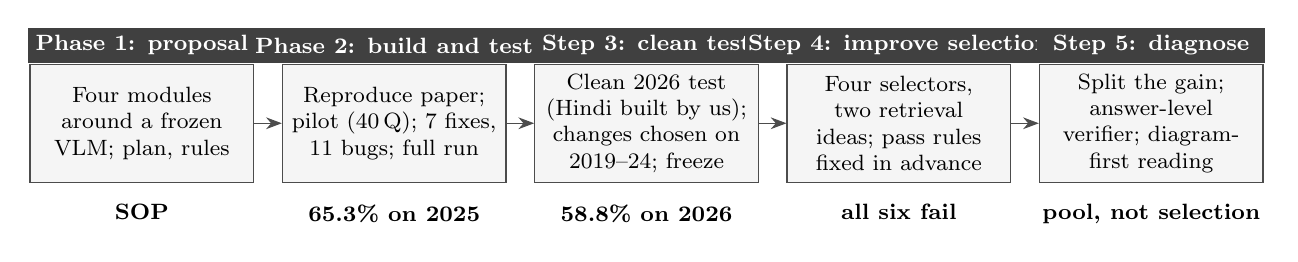
\begin{tikzpicture}[font=\footnotesize, node distance=3.5mm,
  st/.style={draw=black!70, fill=black!4, align=center, minimum height=15mm, text width=27mm,
  inner sep=2pt}, hd/.style={fill=black!75, text=white, font=\footnotesize\bfseries,
  minimum width=29mm, minimum height=4.5mm, inner sep=1pt},
  res/.style={font=\footnotesize\bfseries, align=center}, arr/.style={-{Stealth[length=2mm]}, black!70}]
\node[st] (a) {Four modules around a frozen VLM; plan, rules};
\node[st, right=of a] (b) {Reproduce paper; pilot (40\,Q); 7 fixes, 11 bugs; full run};
\node[st, right=of b] (c) {Clean 2026 test (Hindi built by us); changes chosen on 2019--24; freeze};
\node[st, right=of c] (d) {Four selectors, two retrieval ideas; pass rules fixed in advance};
\node[st, right=of d] (e) {Split the gain; answer-level verifier; diagram-first reading};
\foreach \n/\t in {a/Phase 1: proposal, b/Phase 2: build and test, c/Step 3: clean test,
  d/Step 4: improve selection, e/Step 5: diagnose}
  \node[hd, above=0mm of \n] {\t};
\foreach \n/\t in {a/SOP, b/65.3\% on 2025, c/\ThreeAcc\% on 2026, d/all six fail, e/{pool, not selection}}
  \node[res, below=1.5mm of \n] {\t};
\draw[arr] (a) -- (b); \draw[arr] (b) -- (c); \draw[arr] (c) -- (d); \draw[arr] (d) -- (e);
\end{tikzpicture}
\caption{Study design. Phase~2 gave a positive result on 2025, but 2025 had influenced the
design, so the final test was run on 2026. On 2026 the learned selector no longer helped, which
led to Step~4 (new selectors and retrieval variants, each with a fixed pass rule). None of them
passed, and Step~5 then measured which parts of the system the gain comes from. Steps 4 and 5
took place after the freeze, so their results on the test years are marked post-hoc.}
\label{fig:design}
\end{figure*}

% ==============================================================================================
\section{Related work}
\textbf{Benchmarks.} mmJEE-Eval~\cite{mmjee} evaluates 17 models on JEE questions given only as
images, and it also includes a contamination test and a study of single-pass self-correction.
JEEBench~\cite{jeebench} (text) and OlympiadBench~\cite{olympiadbench} (bilingual olympiad
problems) are related benchmarks.
\textbf{Tool use.} Program-of-thought prompting~\cite{pot} and PAL~\cite{pal} let the model hand
arithmetic to an interpreter.
\textbf{Sampling and voting.} Self-consistency~\cite{selfconsistency} samples several chains of
thought and takes a majority vote.
\textbf{Self-correction.} Self-Refine~\cite{selfrefine} and CRITIC~\cite{critic} alternate
between critique and revision. Huang et al~\cite{cannotselfcorrect} found that models often
cannot correct themselves when no outside signal is available.
\textbf{Verifiers.} Outcome and process verifiers~\cite{cobbe,lightman} rank sampled solutions and
are usually large trained models.
\textbf{Retrieval.} Retrieval-augmented generation~\cite{rag} supplies the model with external
context.

% ==============================================================================================
\section{Data and evaluation protocol}\label{sec:data}
\textbf{Benchmark.} An mmJEE-Eval item is a single image holding the question, its options and
any figure, together with metadata (subject, question type, year, language and the gold answer).
There are four question types (numerical, single-correct MCQ, multiple-correct MCQ and
matching), and 30.3\% of the questions can not be answered without the diagram.

\textbf{Splits.} The data is split by exam year (Table~\ref{tab:splits}). The years 2019--2024
(1{,}270 questions) are used for training and development, and 2024 serves as the dev year. The
2025 exam (\NPost{} questions) was our test year in Phase~2. It was later used for the pilot,
it influenced several design decisions and the model may have seen it, so every 2025 number
reported after Phase~2 is marked as post-hoc.

\textbf{Clean test year.} JEE Advanced 2026 took place after Qwen3-VL was released. The dataset
has its 102 English questions, and we added the 102 Hindi versions ourselves. Each Hindi question
was cropped from the official hindi paper, matched to its English twin by paper, subject and
question number, and given the answer from the English key. An automatic check confirmed every
pairing, and 14 crops, among them all size outliers, were inspected by hand. While doing this we
found and fix three bugs in our parser; in one of them, the Hindi word for ``part'' inside a
physics question had been read as a section heading. Fig.~\ref{fig:example} shows one pair. Our
crops do not look exactly like the dataset images, and for this reason we also give results
separately for each language.

\begin{table}[!t]
\centering\footnotesize
\caption{Data splits (questions; each year has English and Hindi twins).}
\label{tab:splits}
\begin{tabular}{@{}llrP{3.45cm}@{}}
\toprule
Years & Role & Qs & Used for \\
\midrule
2019--2024 & train / dev & 1{,}270 & verifier data, knowledge base; 2024 = dev year \\
2025 & Phase-2 test & \NPost & Phase-2 results; post-hoc afterwards \\
2026 & clean test & \NTest & final results (Hindi built by us) \\
\bottomrule
\end{tabular}
\end{table}

\begin{figure*}[t]
\centering
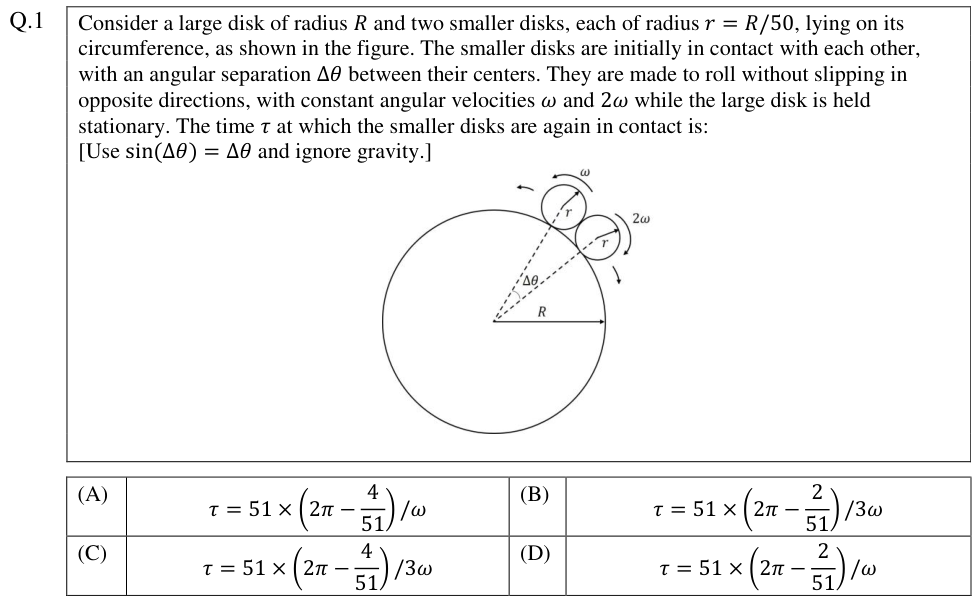
\includegraphics[width=0.47\textwidth]{q2026_en.png}\hfill
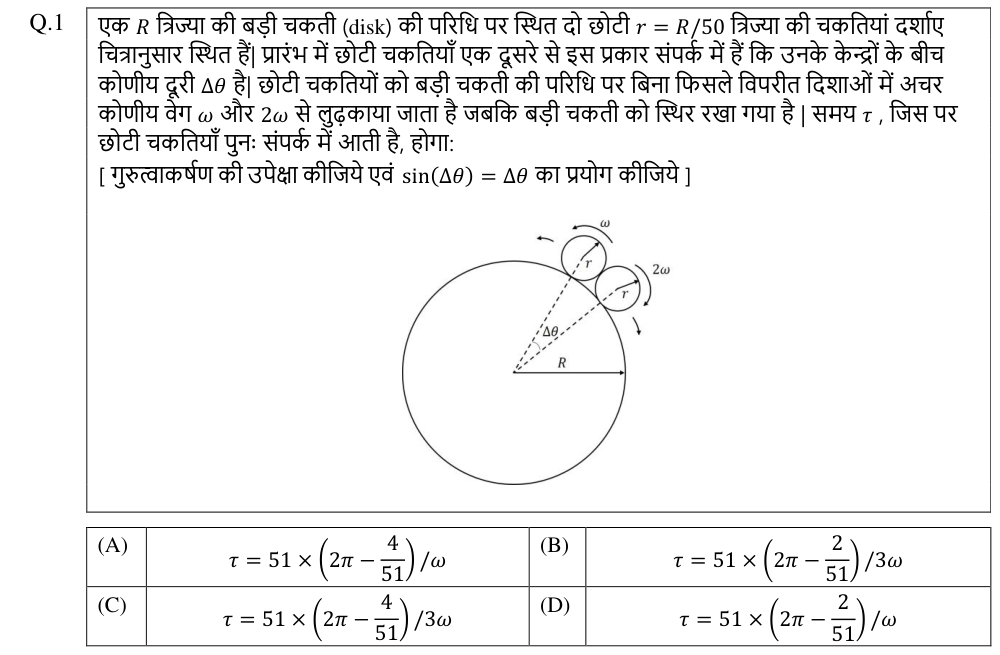
\includegraphics[width=0.47\textwidth]{q2026_hi.png}
\caption{A question from the clean year (JEE Advanced 2026, Paper~1, Physics Q1). Left: the English
image from the dataset. Right: the Hindi version we cropped from the official paper. The model
receives only the image, so it has to read the text, formulas, options and diagram itself.}
\label{fig:example}
\end{figure*}

\textbf{Scoring.} The functions \texttt{extract\_answer} and \texttt{is\_answer\_correct} are
taken from the base paper without changes, and a unit test confirms that every gold answer is
scored as correct. Matching questions are scored in the same way as single correct MCQs. For
rows with several samples, Pass@1 is the average accuracy over the samples. For rows that select
one answer, we report the accuracy of that answer.

\textbf{Compute matching.} Self-consistency (SC) is a majority vote over plain chain-of-thought
(CoT) answers. We draw 20 CoT samples per question and, for each system, use the smallest number
of them whose generated tokens add up to at least the system's own token count.

\textbf{Leakage control.} Test questions and their twins never appear in a training pool.
Knowledge-base entries that are close to any 2025 or 2026 question were deleted, and no 2025 or
2026 data was used when the final system was frozen.

% ==============================================================================================
\section{Proposed method}\label{sec:method}
\begin{figure*}[t]
\centering
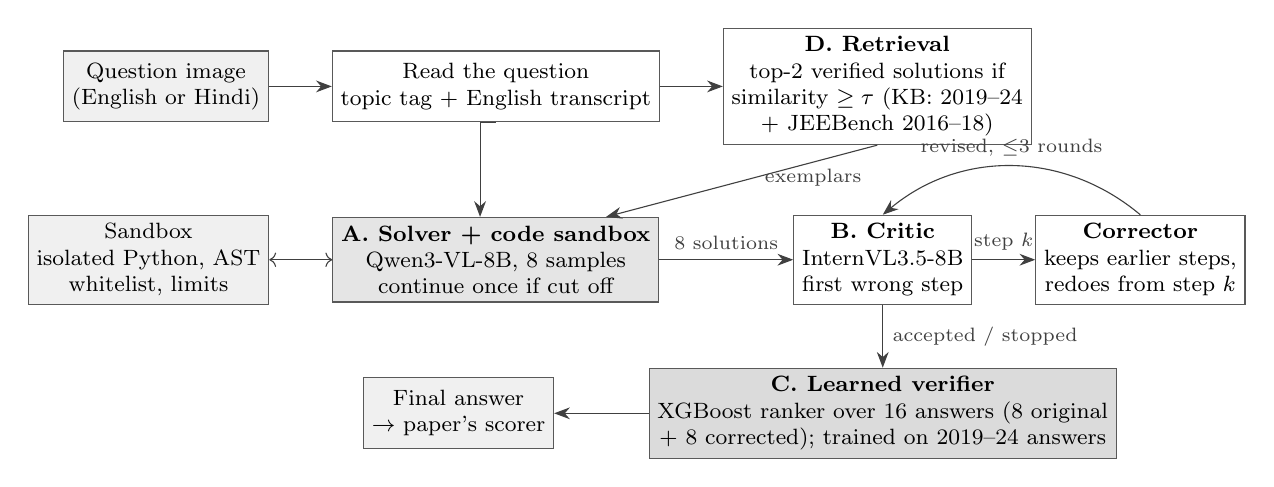
\begin{tikzpicture}[font=\footnotesize, node distance=4mm and 8mm,
  box/.style={draw=black!65, fill=#1, align=center, minimum height=9mm, inner sep=3pt},
  box/.default=white, arr/.style={-{Stealth[length=2mm]}, black!75},
  new/.style={font=\scriptsize\itshape, text=black!60}]
\node[box=black!6] (img) {Question image\\(English or Hindi)};
\node[box, right=of img] (tag) {Read the question\\topic tag + English transcript};
\node[box, right=of tag] (kb) {\textbf{D. Retrieval}\\top-2 verified solutions if\\similarity $\ge\tau$ (KB: 2019--24\\+ JEEBench 2016--18)};
\node[box=black!10, below=12mm of tag, minimum width=38mm] (solver)
  {\textbf{A. Solver + code sandbox}\\Qwen3-VL-8B, 8 samples\\continue once if cut off};
\node[box=black!6, left=of solver] (exec) {Sandbox\\isolated Python, AST\\whitelist, limits};
\node[box, right=17mm of solver] (critic) {\textbf{B. Critic}\\InternVL3.5-8B\\first wrong step};
\node[box, right=of critic] (corr) {\textbf{Corrector}\\keeps earlier steps,\\redoes from step $k$};
\node[box=black!14, below=8mm of critic, minimum width=42mm] (ver)
  {\textbf{C. Learned verifier}\\XGBoost ranker over 16 answers (8 original\\+ 8 corrected); trained on 2019--24 answers};
\node[box=black!6, left=12mm of ver] (out) {Final answer\\$\to$ paper's scorer};
\draw[arr] (img) -- (tag); \draw[arr] (tag) -- (kb);
\draw[arr] (kb.south) -- node[right, pos=0.45]{\scriptsize exemplars} ([xshift=14mm]solver.north);
\draw[arr] (tag.south) -- ([xshift=-2mm]solver.north |- tag.south) -- ([xshift=-2mm]solver.north);
\draw[arr, <->] (exec) -- (solver);
\draw[arr] (solver) -- node[above]{\scriptsize 8 solutions} (critic);
\draw[arr] (critic) -- node[above]{\scriptsize step $k$} (corr);
\draw[arr] (corr.north) to[bend right=40] node[above]{\scriptsize revised, $\le$3 rounds} (critic.north);
\draw[arr] (critic) -- node[right]{\scriptsize accepted / stopped} (ver);
\draw[arr] (ver) -- (out);
\end{tikzpicture}
\caption{The framework around the frozen VLM. The verifier (C) is the only trained part, and it
is trained on automatically labelled answers from 2019--2024.}
\label{fig:arch}
\end{figure*}

\subsection{Modules}
The full prompts are reproduced in Appendix~\ref{app:prompts}.
\textbf{A. Code sandbox (program of thought).} The solver writes its solution as numbered steps
and places every calculation in a \texttt{python} block. Each block is executed in a separate
subprocess (\texttt{python -I}) after an AST check that admits math, NumPy, SymPy and SciPy and
rejects any file or network access, with limits on time, memory and output size. The output is
inserted into the solution and generation than continues. Before a block runs, the earlier
blocks of the same solution are executed again so that their variables are available. When the
solution ends without a \verb|\boxed{}| answer, a plain CoT answer is used instead.

\textbf{B. Agentic correction.} The critic, InternVL3.5-8B, comes from a different model family
than the solver. It reads a solution and either names the first wrong step or replies
\texttt{NO\_ERROR}. The corrector, which is the solver model again, keeps the steps before the
flagged one and works out the remainder anew. Atmost three rounds are run, and the loop ends
early if the critic accepts the solution or the answer stays the same for two rounds. If a critic
reply is cut off, we append a short cue asking for the decision and let the critic continue
greedily for a few tokens (\emph{verdict forcing}).

\textbf{C. Learned verifier.} The scorer can mark every answer sampled on 2019--2024 as right or
wrong, so labelled training data is available without manual annotation (in Phase~2, 10{,}160
answers, of which 45.5\% were correct). The features are hand crafted: length, number of steps,
whether the code ran, truncation, hedging words, format, agreement with the other answers in the
pool and in each half of it, critic flags, number of rounds and whether the answer changed. In
Phase~2 a sentence embedding was also used. The verifier scores all 16 candidates (the 8 original
solutions and their 8 corrected versions) and returns the answer with the highest score.

\textbf{D. Retrieval.} The model first writes a one-line tag naming the topic and the method. We
embed this tag with bge~\cite{bge}, search with FAISS~\cite{faiss} and take at most two verified worked solutions of the same subject from earlier
years. They are added to the prompt as examples of the method only when their similarity is above
a threshold $\tau$, so that weakly related problems are left out.

\subsection{From the Phase-2 system to the final system}
We chose every change below using only 2019--2024 data, with a rule set before testing: a
change is kept only if it raises accuracy on the 2024 dev year and the lower end of its 95\% CI
is above zero (Table~\ref{tab:devab}).
\begin{itemize}
\item \emph{Transcript.} The model first writes the question out in English, translating it if
it is in Hindi. The solver then gets this text along with the image.
\item \emph{Continuation.} If an answer runs out of tokens, we let it go on once for up to
4{,}096 more tokens. We do this for every row, the baselines too so the comparison stays fair.
\item \emph{Hybrid retrieval.} The search uses the problem text as well as the tag, JEEBench
2016--2018 is added to the knowledge base, and $\tau$ is set with leave-one-year-out (LOYO) tests.
More questions now get examples (\RagCovTwo\% $\to$ \RagCovThree\% under LOYO), the examples are
as good as before, and dev accuracy stays the same.
\item \emph{Ranking verifier.} An XGBoost model that ranks the answers of a pool against each
other, chosen by LOYO on 2019--2024. It is trained on pools that also hold corrected answers,
just like the test pools. Under LOYO it picks a right answer in \VerLoyo\% of pools, against
\VerLoyoMaj\% for majority voting; the best possible (oracle) is \VerLoyoOracle\%.
\item \emph{Correction gate.} A corrected answer replaces the original only if the verifier's
score goes up by more than $\delta{=}$\GateDelta, with $\delta$ picked on other years. The gate
has its own row in the results, but the final answer is still the verifier's pick from the full
pool.
\end{itemize}
We froze the configuration and commited it to the repository before the first 2026 run.

\begin{table}[!t]
\centering
\footnotesize
\caption{Dev A/B tests on 2024 (204 questions) that decided the freeze. Rule fixed in advance: include iff $\Delta>0$ and the CI lower bound $>0$.}
\label{tab:devab}
\setlength{\tabcolsep}{3.5pt}
\begin{tabular}{lrrr}
\toprule
Arm & Base & Arm & $\Delta$ [95\% CI] \\
\midrule
Transcript block (PoT) & 50.2 & 55.1 & +4.9 [+1.8, +8.2] \\
Continuation (PoT) & 50.2 & 52.6 & +2.3 [+1.0, +3.7] \\
Continuation (CoT) & 48.5 & 54.9 & +6.4 [+2.5, +10.8] \\
Retrieval, Phase-2 recipe & 50.2 & 50.4 & +0.2 [$-$2.3, +2.9] \\
Retrieval, hybrid + JEEBench & 50.2 & 50.6 & +0.3 [$-$2.1, +3.0] \\
\bottomrule
\end{tabular}
\end{table}


% ==============================================================================================
\section{Experimental setup}
Qwen3-VL-8B-Instruct~\cite{qwen3vl} is the solver and also writes the transcript, and
InternVL3.5-8B~\cite{internvl35} is the critic. Both are frozen and quantised to 4 bits with AWQ.
the base paper's model, Qwen2.5-VL-7B, is used for the reproduction and for one bridge
experiment. Each lab PC has one NVIDIA RTX 3060 (12\,GB) and 15\,GB of RAM, and the models are
served with vLLM~\cite{vllm} in offline batch mode, one model at a time.

All rows use temperature 0.7, top-$p$ 0.8, top-$k$ 20 and a limit of 4{,}096 tokens per call. We
draw 20 CoT samples per question and 8 samples for PoT and correction. Each model call is stored
in an SQLite cache with a fixed seed, so a run that stops halfway can be resumed and gives the
same results.

% ==============================================================================================
\section{Phase 2: building and testing on 2025}\label{sec:p2}
\textbf{Setup check.} We first compared our evaluation code with a published number. Using the
paper's prompts and scorer, Qwen2.5-VL-7B obtains 13.8$\pm$1.9\% over 10 runs (CI 10.7--17.3),
close to the 12.4$\pm$1.9\% given in the paper. Qwen3-VL-8B, our solver, obtains 43.4\% with one
answer (16 runs) and 53.7\% with a majority vote over 16 answers. Hindi questions are 10 points
below English ones and diagram questions 18 points below text-only ones, and 40\% of the answers
reach the 4{,}096-token limit.

\textbf{Pilot.} We then ran all modules end to end on 40 test questions. Accuracy went up with
each module (29.5\% for a single answer, 41.2\% with the code sandbox and 57.5\% for the full
framework), and the full framework was 22.5 points above matched SC (CI [7.5, 37.5]). Forty
questions gives only a rough first estimate, and the pilot was more useful for finding problems.
We read 1{,}520 solution traces and 640 correction chains and found seven problems in the method
(Table~\ref{tab:fixes}). Before the big GPU runs we went through the code again and found 11 more
bugs, for example a crash in the verifier's cross-validation, features that were computed
differently in training and at test time, and confidence intervals that ignored the link between
twin questions. Each fix is covered by a regression test.

\begin{table}[!t]
\centering\scriptsize
\caption{Problems found in the pilot traces and their fixes.}
\label{tab:fixes}
\setlength{\tabcolsep}{2.5pt}
\begin{tabular}{@{}P{1.55cm}P{2.75cm}P{3.9cm}@{}}
\toprule
Problem & Evidence & Fix and effect \\
\midrule
Code state lost & 47 \texttt{NameError}s; each block ran in a fresh process & Replay earlier blocks first; 0 errors \\
Library blocked & 86 blocks needed SciPy & SciPy allowed (no file I/O); 0 blocked \\
No critic verdict & 76 replies cut off while re-solving & Short check + verdict forcing: 1 of 501 unparsed; detection 35\%$\to$56\% \\
Many fallbacks & 480 of 539 fallbacks were long reasoning loops & Forcing an answer tested: 21.9\% vs.\ 30.0\% $\Rightarrow$ rejected \\
SC too small & system used $\approx$18 answers' tokens, 16 drawn & 20 CoT samples per question \\
Selector = vote & dev pick equal to majority & reported; 8$\times$ more training data \\
Batch aborted & one 12{,}303-token prompt & retry request by request \\
\bottomrule
\end{tabular}
\end{table}

\begin{table}[!t]
\centering
\footnotesize
\caption{Phase-2 framework on JEE Advanced 2025 (190 questions; the Phase-2 test year). Rows add one module at a time from the code sandbox. Accuracy in \%, 95\% cluster-bootstrap CI; tokens are generated tokens per question.}
\label{tab:p2}
\setlength{\tabcolsep}{3pt}
\begin{tabular}{lrrcr}
\toprule
Configuration & Acc. & Num. & 95\% CI & Tok./q \\
\midrule
Baseline (single-pass CoT) & 43.2 & 40.2 & 37.0--49.6 & 2.7k \\
Self-consistency (matched, $n{=}20$) & 53.2 & 51.2 & 44.2--62.6 & 54.2k \\
+ Code sandbox (PoT) & 48.2 & 50.4 & 41.4--54.9 & 3.5k \\
+ Correction, same-model critic & 51.2 & 55.1 & 44.6--58.0 & 6.1k \\
+ Correction, cross-model critic & 51.3 & 53.0 & 44.5--58.1 & 6.4k \\
+ Learned verifier & 63.2 & 66.7 & 55.3--71.6 & 51.5k \\
\textbf{+ Retrieval = full framework} & \textbf{65.3} & 69.0 & 57.4--73.7 & 54.1k \\
\bottomrule
\end{tabular}
\end{table}


\textbf{Full run on 2025.} Table~\ref{tab:p2} and Fig.~\ref{fig:p2} show the results as modules are
added one by one. The full framework reaches 65.3\%, against 43.2\% for one answer, and is 12.1
points above matched SC (CI [4.2, 20.5], McNemar $p{=}0.001$). There are 35 question that only
the framework solves and 12 that only SC solves. With the code sandbox, accuracy on numerical
questions goes from 40.2\% to 50.4\%, and overall accuracy rises by 5.0 points ($p{=}0.012$). The
verifier gives the largest single increase (+11.8, CI [6.8, 16.6]), while retrieval adds 2.1
points. A single CoT sample per question scores 43.9\% on 2019--2024
and 42.6\% on 2025, which gives no indication that the model had memorised 2025.

\begin{figure}[t]
\centering
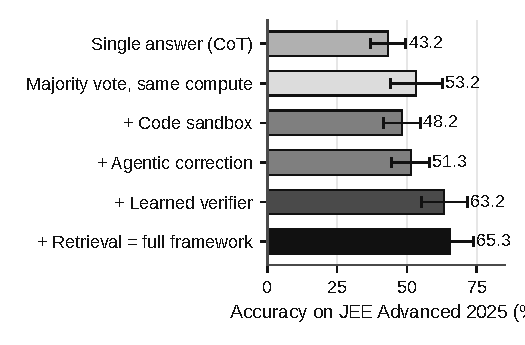
\includegraphics[width=\columnwidth]{phase2_ladder.pdf}
\caption{Phase-2 framework on 2025, adding one module at a time (95\% CIs).}
\label{fig:p2}
\end{figure}

\textbf{Open questions after Phase 2.} Three observations guided the rest of the study. First,
on the 2025 pool the Phase-2 verifier picked 65.3\%, almost the same as a plain majority vote over
the same 16 answers (65.8\%, oracle 85.3\%). Most of the gain therefore came from the variety of
the pool and little from the choice among its answers. Second, retrieval was used for only 30 of
the 190 questions. Third, 2025 was no longer a clean test year
(Sec.~\ref{sec:data}).

% ==============================================================================================
\section{Results and analysis on the clean 2026 test}\label{sec:main}
Fig.~\ref{fig:main} shows the results for both frameworks as modules are
added. The final framework reaches \textbf{\ThreeAcc\%}, compared with \ThreeBase\% for one
answer, an increase of \ThreeGain{} points. It generates about \ThreeTok{} tokens per question,
which buys \ThreeScN{} samples for matched SC, and SC with these samples reaches \ThreeSc\%. The
framework is \ThreeVsSc{} points higher (CI [\ThreeVsScLo, \ThreeVsScHi]); it solves \ThreeFwOnly{}
questions that SC gets wrong, while SC solves \ThreeScOnly{} that the framework gets wrong. The
Phase-2 framework, run again without changes, reaches \TwoAcc\% and is \TwoVsSc{} points above
its own matched SC ($p{=}$\TwoVsScP). Our main claim, that the framework does better than
majority voting at the same compute, thus also holds on an exam written after the model was
released. In Fig.~\ref{fig:compute}, every row of the framework lies above the SC curve at the
corresponding cost.

\begin{figure*}[t]
\centering
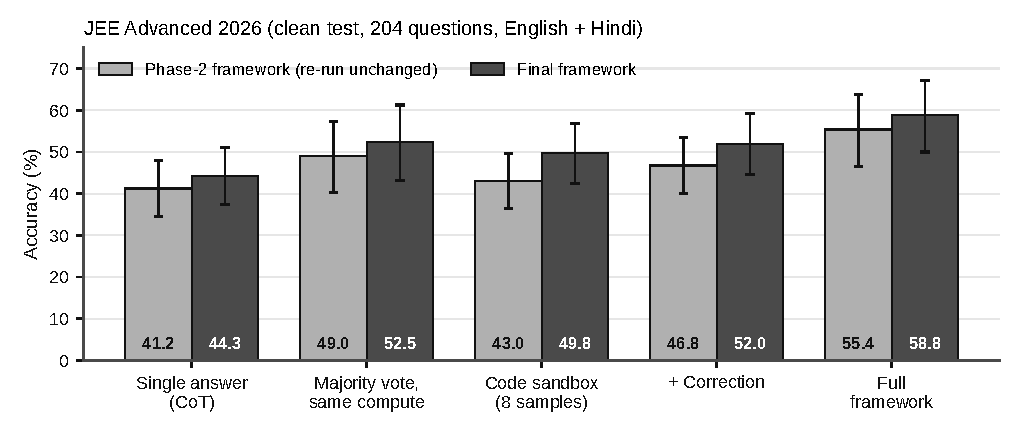
\includegraphics[width=0.86\textwidth]{main_2026.pdf}
\caption{Clean 2026 test: matching rows of the Phase-2 framework (re-run unchanged) and the final
framework, with 95\% cluster-bootstrap CIs. Majority vote uses the same number of generated tokens
as the corresponding full framework.}
\label{fig:main}
\end{figure*}

\begin{figure}[t]
\centering
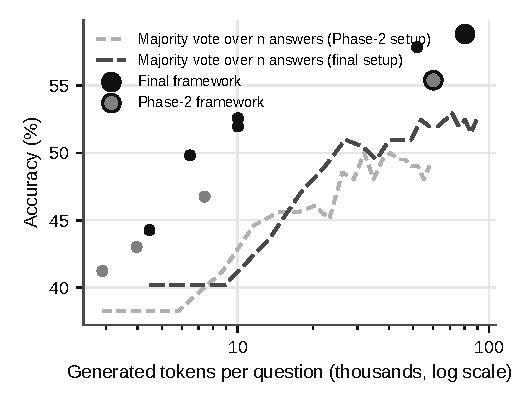
\includegraphics[width=\columnwidth]{compute_2026.pdf}
\caption{2026: accuracy vs.\ generated tokens per question. Dashed: majority vote over $n$ CoT
answers. Dots: rows of Fig.~\ref{fig:main}; large dots: the full frameworks.}
\label{fig:compute}
\end{figure}

\begin{table}[!t]
\centering
\scriptsize
\caption{Paired comparisons (cluster bootstrap; McNemar counts questions only $a$ / only $b$ gets right; it is meaningful for single-answer rows only, as Pass@1 rows are rounded per question). $^\dagger$post-hoc.}
\label{tab:cmp}
\setlength{\tabcolsep}{2.5pt}
\begin{tabular}{lrrrr}
\toprule
Comparison ($a$ vs.\ $b$) & $\Delta$ [95\% CI] & P($\Delta{\le}0$) & $a$/$b$ & $p$ \\
\midrule
2026 final vs.\ Phase-2 framework & +3.4 [$-$1.5, +8.8] & 0.113 & 16/9 & 0.230 \\
2026 final vs.\ Phase-2 PoT & +6.8 [+3.6, +10.0] & 0.000 & 27/3 & $<$0.001 \\
2026 CoT with continuation vs.\ CoT & +3.0 [+1.7, +4.5] & 0.000 & 6/3 & 0.508 \\
2026 gated vs.\ ungated correction & +0.6 [$-$0.4, +1.5] & 0.122 & 4/1 & 0.375 \\
2026 verifier pick vs.\ mean PoT answer & +9.0 [+5.8, +12.4] & 0.000 & 17/0 & $<$0.001 \\
2025$^\dagger$ final vs.\ Phase-2 framework & +6.8 [+1.1, +12.1] & 0.012 & 21/8 & 0.024 \\
2025$^\dagger$ final vs.\ Phase-2 PoT & +8.1 [+4.8, +11.6] & 0.000 & 30/7 & $<$0.001 \\
\bottomrule
\end{tabular}
\end{table}


\textbf{Final vs.\ Phase-2 framework.} The paired tests are in Table~\ref{tab:cmp}. The solver of the
final system is clearly stronger. Its PoT answers are \PotVsDiff{} points better than those of the
Phase-2 system (CI [\PotVsLo, \PotVsHi]), and continuation on its own adds \ExtVsDiff{} points to
CoT. For the complete frameworks the difference is \VsDiff{} points (CI [\VsLo, \VsHi],
$p{=}$\VsP), which is not significant with \NTest{} questions. On the post-hoc 2025 set the same
comparison gives \PostVsDiff{} (CI [\PostVsLo, \PostVsHi]). The verifier accounts for most of the
difference between the two years (Sec.~\ref{sec:ver}).

\begin{figure*}[t]
\centering
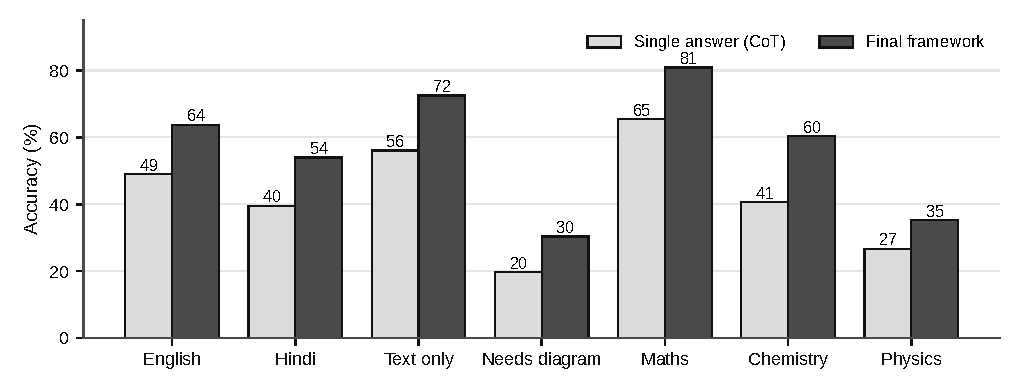
\includegraphics[width=0.86\textwidth]{breakdown_2026.pdf}
\caption{2026 accuracy by group: one CoT answer vs.\ the final framework.}
\label{fig:bd}
\end{figure*}

\textbf{Results by group.} Accuracy improves in every group (Fig.~\ref{fig:bd}). On 2026 English questions reach \ThreeEn\% and
Hindi questions \ThreeHin\%, and text-only questions reach \ThreeTxt\% while diagram questions
reach only \ThreeImg\%. The code sandbox and correction improve the reasoning, but they cannot
help when the model has read the figure wrongly. Some of the Hindi gap on 2026 could also be
caused by our own crops.


\subsection{Correction on clean data}\label{sec:corr}
\begin{table}[!t]
\centering
\scriptsize
\caption{Correction loop, paper-style metacognition (\%). EP: wrong solutions flagged in round 1; EC: round-1 fixes among detected; FA: correct solutions flagged. W$\to$R / R$\to$W: answer flips after all rounds.}
\label{tab:corr}
\setlength{\tabcolsep}{2.5pt}
\begin{tabular}{lrrrrrrr}
\toprule
Run & Chains & Acc. & EP & EC & FA & W$\to$R & R$\to$W \\
\midrule
2026 Ph.\,2, PoT + corr. & 1632 & 43.0$\to$46.8 & 67.5 & 9.7 & 23.6 & 76 & 15 \\
2026 Ph.\,2, full & 1632 & 44.7$\to$48.8 & 69.0 & 10.8 & 25.2 & 83 & 16 \\
2026 final & 1632 & 49.8$\to$52.0 & 52.9 & 13.2 & 19.9 & 68 & 33 \\
2025$^\dagger$ final & 1520 & 56.2$\to$57.9 & 40.3 & 13.1 & 23.3 & 46 & 21 \\
2025 Ph.\,2, PoT + corr. & 1520 & 48.2$\to$51.3 & 59.3 & 13.3 & 25.7 & 87 & 39 \\
2025 Ph.\,2, full & 1520 & 50.9$\to$54.7 & 60.7 & 15.7 & 28.6 & 87 & 29 \\
\bottomrule
\end{tabular}
\end{table}

Table~\ref{tab:corr} uses the measures defined in the base paper. In round~1 the critic flags
\EpThree\% of the wrong solutions of the final system, and \EcThree\% of the flagged errors are
fixed in that round. Counting all rounds, 14--19\% of the detected errors end with a correct
answer (Fig.~\ref{fig:corr}). The base paper reports 1.1--5.2\% for single-pass correction. We
think the difference come from three sources: the feedback points to a specific step, it comes
from a second model, and the solver can check its numbers in the sandbox. The critic also flags
\FaThree\% of the \emph{correct} solutions, and some of these are then changed from right to
wrong. Since the final solver is stronger, fewer of its solutions are wrong to begin with, and
the absolute gain from correction is smaller than in Phase~2.

\begin{figure*}[t]
\centering
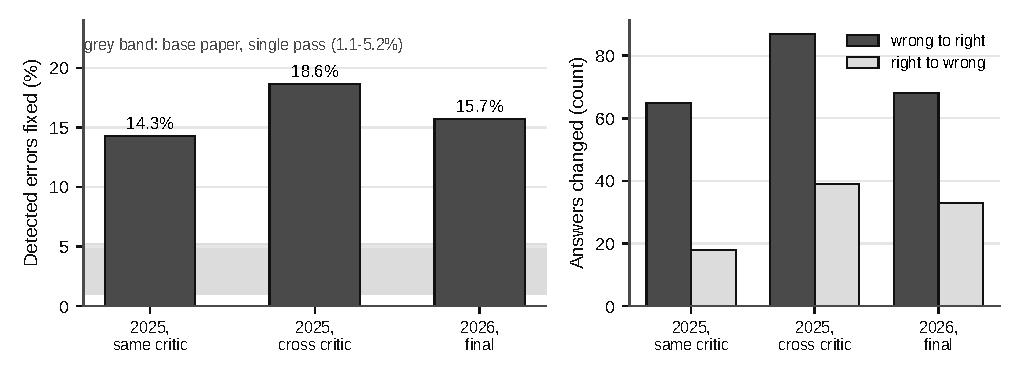
\includegraphics[width=0.8\textwidth]{correction.pdf}
\caption{Correction loop. Left: share of detected errors that are correct after up to three rounds;
the grey band is the base paper's single-pass rate of 1.1--5.2\%. Right: answers changed by
correction, in each direction.}
\label{fig:corr}
\end{figure*}

On 2026 the correction gate reduces the right$\to$wrong changes from \GateRtwU{} to \GateRtwG{}
and keeps most of the useful ones (wrong$\to$right goes from \GateWtrU{} to \GateWtrG). Accuracy
per chain changes from \GateAccU\% to \GateAccG\% (\GateVsDiff{}, CI [\GateVsLo, \GateVsHi]). This
difference is not significant, because the gate also rejects some correct fixes.

\subsection{The verifier as a classifier and as a selector}\label{sec:ver}
\begin{table}[!t]
\centering
\footnotesize
\caption{Primary verifier on its own 16-answer test pool: AUC and accuracy of the picked answer vs.\ pool baselines (\%).}
\label{tab:ver}
\setlength{\tabcolsep}{3.5pt}
\begin{tabular}{llrrrrr}
\toprule
Pool & Verifier & AUC & Pick & Maj. & Rand. & Oracle \\
\midrule
2026 final & XGBoost ranker & 0.902 & \textbf{58.8} & 59.3 & 50.9 & 79.4 \\
2026 Phase-2 & LogReg, all feat. & 0.913 & \textbf{55.4} & 53.9 & 46.7 & 76.5 \\
2025$^\dagger$ final & XGBoost ranker & 0.872 & \textbf{72.1} & 65.8 & 57.1 & 87.4 \\
2025 Phase-2 & LogReg, all feat. & 0.836 & \textbf{65.3} & 65.8 & 52.8 & 85.3 \\
\bottomrule
\end{tabular}
\end{table}

Judged as a classifier of single answers the verifier carries over well to 2026, with an AUC of
\VerAucTest{} on the 2026 pool (Table~\ref{tab:ver}). Judged by the answer it picks, however, it
brings no gain on the clean year. It picks a right answer for \ThreePick\% of the questions,
while majority voting over the same 16 answers gives \ThreeMaj\% and the oracle \ThreeOracle\%.
On 2025 it was \PostPickVsMaj{} points above majority voting. On 2026 the improvement therefore
comes from the better pool of candidates, produced by the transcript, continuation and
correction, rather than from the selection step. Choosing among the 8 PoT answers alone already
gives \ThreePotVer\%. Before the runs we had noted one possible cause. The verifier was trained on
plain PoT solutions of about \TokTrain{} tokens, whereas the 2026 solutions of the final system
are about \TokTest{} tokens long because of the transcript and the continuation. This explanation
is tested in Sec.~\ref{sec:sel}.

\subsection{Checks on the evaluation}
\textbf{Memorisation probe.} When asked for the answer only (64 tokens, no reasoning), Qwen3-VL
scores \ProbeOldLo--\ProbeOldHi\% on 2019--2024, \ProbeTwentyFive\% on 2025 and \ProbeTwentySix\%
on 2026 (Fig.~\ref{fig:probe}). The score on the clean year is not lower than on the earlier
years, so the probe shows no sign of memorisation.

\begin{figure}[t]
\centering
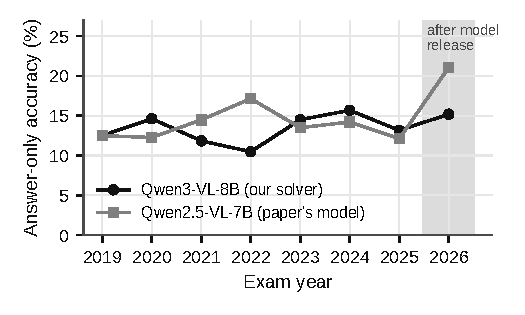
\includegraphics[width=\columnwidth]{memorisation_probe.pdf}
\caption{Answer-only accuracy by exam year. 2026 is after both models' release.}
\label{fig:probe}
\end{figure}

\textbf{Bridge to the papers model.} With Qwen2.5-VL-7B the framework gives no improvement. One
answer scores \QBase\%, matched SC \QSc\% and the framework \QFull\% (\QVsSc{} against SC, CI
[\QVsScLo, \QVsScHi]). At an accuracy of about 14\% most candidates are wrong, and agreement
between answers, the critic and the verifier then provide little useful information. The
framework only helps when the solver is right reasonably often.

\textbf{Post-hoc 2025.} On 2025 the final framework reaches \PostAcc\%, compared with
\PostTwoAcc\% for the Phase-2 run, and it is \PostVsSc{} points above matched SC. The gaps are
larger on 2025 than on 2026, which fits with some optimism on a year that influenced the design.

% ==============================================================================================
\section{Can selection or retrieval be improved?}\label{sec:sel}
After the main result we worked on its two weak points, selection and retrieval. By this time we
had already seen results on both test years, so all 2025 and 2026 numbers in this section and the
next are post-hoc. Every choice was still made on 2019--2024 data, following a plan committed
before the runs.

\begin{figure*}[t]
\centering
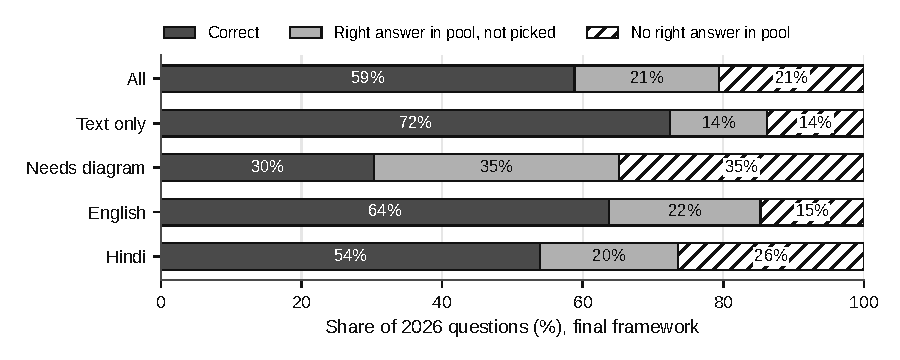
\includegraphics[width=0.78\textwidth]{errors_2026.pdf}
\caption{Outcome of each 2026 question for the final framework: solved, right answer present in
the pool but not picked, or no right answer in the pool.}
\label{fig:err}
\end{figure*}

\textbf{Error analysis.} Of the 204 questions, 120 are solved. For \VfErrMiss{} the pool holds a
right answer that the selector does not pick, and for \VfErrNever{} the pool holds no right answer
at all (Fig.~\ref{fig:err}). In the pools where the selector misses, only \VfErrShare\% of the
candidates are right, so the right answer is clearly in the minority. Most of these errors are on
diagram questions. Among them, \VfImgMiss\% are selector misses and the same share never get a
right answer into the pool, compared with \VfTxtMiss\% in each category for text-only questions.
The difference in solution length does not explain the drop. The final system's solutions are
longer than the training solutions in both years (\VfTokTwentyFive{} and \VfTokTwentySix{} tokens
against \VfTokTrain, with small standardised differences of \VfSmdTwentyFive{} and
\VfSmdTwentySix), and yet the verifier is better than majority voting on 2025
(\VfVerMajTwentyFive) and not on 2026 (\VfVerMajTwentySix).

\begin{table}[!t]
\centering\footnotesize
\caption{New selectors: pick accuracy (\%) under LOYO on the 16-answer training pools
(2019--2024, 242 pools; no test data). Pass rule (fixed in advance): beat the frozen ranker on
every pool type. Ranker LOYO noise is about 1 point.}
\label{tab:sel}
\begin{tabular}{lrl}
\toprule
Selector & LOYO pick & Rule \\
\midrule
Frozen ranker (final framework) & \VfRef & reference \\
Ranker without length features & \VfNoLen & fail \\
Fine-tuned neural verifier (ModernBERT) & \VfNeural & fail \\
Ranker + neural score (stacked) & \VfStacked & fail \\
Ranker with \VfXRows{} matched training answers & \VfXRef & fail \\
Answer-level verifier (Sec.~\ref{sec:diag}) & \VbAMean & fail \\
\midrule
Majority vote & \VfMaj & \\
Oracle & \VfOracle & \\
\bottomrule
\end{tabular}
\end{table}

\textbf{New selectors} (Table~\ref{tab:sel}). We tried four variants. The first is the ranker
with its length features removed, which tests the length explanation directly; its accuracy goes
down. The second is a neural verifier, a ModernBERT-base cross-encoder~\cite{modernbert}
fine-tuned on the English transcript, the answer and the end of the solution (1{,}024 tokens),
with one fold per training year. It does learn something useful (candidate AUC \VfAuc, between
\VfAucLo{} and \VfAucHi{} across years), and used as a weight in the vote it is better than plain
majority voting, but as a ranker it is worse than the handcrafted model. The third adds the
neural score to the ranker as one more feature. The fourth retrains all of the above with
\VfXRows{} new training answers produced in the style of the final system (398 training
questions, about 30 GPU-hours), so that the training pools look like the test-time solutions.
None of them meet its pass rule and as planned, none was evaluated on the test years.

\begin{table}[!t]
\centering
\scriptsize
\caption{Retrieval variants, paired differences (points, 95\% cluster-bootstrap CI). Top: 2024 dev year with matched seeds, 204 questions, RAG fires on 31. Bottom: post-hoc 2026 PoT with the extended KB ($^\dagger$right column: questions whose retrieval changed). LOYO coverage at proxy precision 0.70: extended KB 13.5\% vs.\ current KB 15.0\%.}
\label{tab:v4rag}
\setlength{\tabcolsep}{2.5pt}
\begin{tabular}{lrr}
\toprule
Comparison & All & RAG fires \\
\midrule
Solutions $-$ no RAG & $-$0.2 [$-$1.0, +0.4] & $-$1.6 [$-$6.2, +2.5] \\
Cards $-$ no RAG & +0.3 [$-$0.2, +0.9] & +2.0 [$-$1.6, +6.2] \\
\textbf{Cards $-$ solutions} & +0.6 [$-$0.1, +1.3] & +3.6 [$-$0.8, +8.5] \\
\midrule
Extended KB $-$ current KB, 2026$^\dagger$ & +0.0 [$-$0.4, +0.4] & +0.0 [$-$6.2, +7.3] \\
\bottomrule
\end{tabular}
\end{table}


\textbf{Retrieval} (Table~\ref{tab:v4rag}). In these runs the retrieval arms reuse the seeds of the
run without retrieval. A question that receives no examples therefore produces exactly the same
output, and the effect is measured only on the questions where retrieval is used (\VfFired{} of
the \VfDevQ{} dev questions). We tested two ideas. The first replaces the worked solution with a
short \emph{method card} that states the method, when it applies, a plan, the key equations and a
common mistake, and leaves out the answer. On the questions with retrieval, cards are \VfCardSol{}
points better than solutions (P($\Delta{\le}0$)${=}$\VfCardSolP). The lower end of the interval is
below zero, so cards were not adopted under our rule. The second idea extends the knowledge base
with \VfOlyEntries{} verified OlympiadBench solutions, which are released under Apache-2.0. LOYO
coverage then falls from \VfCovThree\% to \VfCovFour\%, because the new close neighbours push up
the tuned threshold while being retrieved only \VfOlyHits{} times themselves. On 2026, retrieval
changes for \VfKbChanged{} questions and the accuracy stays the same. We didnot use coaching
material, because of its licences and the risk of overlap with the test questions.

% ==============================================================================================
\section{Where does the gain come from?}\label{sec:diag}
We ran three last analyses, each with a pass rule fixed beforehand.

\begin{table}[!t]
\centering
\scriptsize
\caption{Where the final framework's gain over matched self-consistency comes from (\%; differences in points, 95\% cluster-bootstrap CI). Pool gain: majority vote on our pool $-$ matched SC; selection gain: verifier pick $-$ majority on the same pool. Frozen verifier and existing pools only. Mixed pools hold both right and wrong answers (number of pools in brackets).}
\label{tab:v4bdecomp}
\setlength{\tabcolsep}{2.5pt}
\begin{tabular}{lrr}
\toprule
 & 2025 & 2026 \\
\midrule
Matched self-consistency & 58.4 & 52.5 \\
Majority vote on our pool & 65.8 & 59.3 \\
Verifier pick & 72.1 & 58.8 \\
\midrule
Pool gain & +7.4 [+0.0, +15.3] & +6.9 [+2.0, +11.8] \\
\textbf{Selection gain} & +6.3 [+1.6, +11.1] & $-$0.5 [$-$2.9, +2.5] \\
Total gain & +13.7 [+5.8, +21.6] & +6.4 [+1.5, +11.3] \\
\midrule
Candidate AUC, all & 0.872 & 0.902 \\
Candidate AUC, mixed pools & 0.796 (129) & 0.748 (121) \\
\bottomrule
\end{tabular}
\end{table}


\textbf{Pool gain and selection gain} (Table~\ref{tab:v4bdecomp}, Fig.~\ref{fig:decomp}). We
split the gain over matched SC into two parts. The \emph{pool gain} is how much a majority vote
on our 16-answer pool beats matched SC, and the \emph{selection gain} is how much the verifier's
pick beats that vote. The pool gain is about the same in both years (\VbPoolTwentyFive{} and
\VbPoolTwentySix{} points), but the selection gain falls from \VbSelTwentyFive{} to
\VbSelTwentySix. The verifier's overall AUC is in fact higher on 2026 (\VbAucAllTwentySix{}
against \VbAucAllTwentyFive), because most of it comes from telling easy questions from hard
ones. Picking only matters in pools with both right and wrong answers, and inside those pools the
mean AUC falls from \VbAucInTwentyFive{} to \VbAucInTwentySix. So a high overall AUC does not mean
that a verifier picks well.

\begin{figure}[t]
\centering
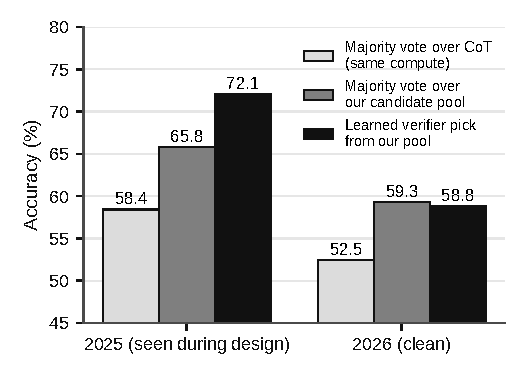
\includegraphics[width=\columnwidth]{decomposition.pdf}
\caption{Decomposition of the gain. In both years a majority vote over our pool is about 7 points
above matched SC. Picking with the verifier adds a further 6.3 points on 2025 and nothing on 2026.}
\label{fig:decomp}
\end{figure}

\textbf{Answer-level verifier.} The ranker scores each solution on its own. We also tried a model
that scores each \emph{distinct answer} in a pool, using features such as its vote share, how many
original and corrected solutions support it, whether their code ran, and the question type
(\VbARows{} answer rows). We kept the setting with the best worst-year LOYO score. It gets
\VbAMean\% (worst year \VbAWorst\%), against \VbARef\% (\VbARefWorst\%) for the ranker and
\VbAMaj\% for majority voting, so it does not pass. Grouping solutions by answer beats voting,
but it loses the per-solution detail that the ranker uses.

\textbf{Diagram-first transcript} (Fig.~\ref{fig:diag}). The usual transcript describes the
figure in one line. We tried a longer reading that lists every label, value with unit, arrow and
axis in the figure, and solved half of each pool from it with the same seeds, so only the
transcript differs. On the 2024 dev year majority@8 changes by \VbBMaj{} points, the rule is not
met, and we did not run it on 2026. Accuracy per answer drops by \VbBSample{} points, mostly on
diagram questions (\VbBImgCur\%$\to$\VbBImgDiag\%), because the longer reading uses up tokens and
more answers get cut off (\VbBTrCur\%$\to$\VbBTrDiag\%). It gives more distinct answers but no
extra right ones (oracle@8 \VbBOrcRef\%$\to$\VbBOrcMulti\%). So the weakness on diagram questions
is not about how the transcript is written: the 8B solver misreads the figure, or reasons wrongly
about it, either way.

\begin{figure*}[t]
\centering
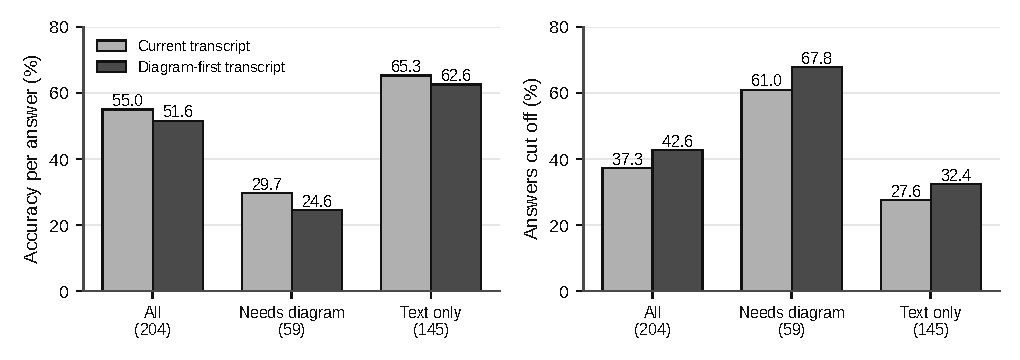
\includegraphics[width=0.8\textwidth]{diagram_first.pdf}
\caption{Diagram-first transcript on the 2024 dev year (samples 4--7, same seeds). Left: accuracy
per answer. Right: share of answers cut off at the token limit.}
\label{fig:diag}
\end{figure*}

% ==============================================================================================
\section{Ablation study}\label{sec:abl}
Fig.~\ref{fig:main} already adds the modules one at a time. Table~\ref{tab:abl} brings together
the experiments in which a single component was switched on or off with everything else held
fixed. The numbers are taken from Tables~\ref{tab:devab}, \ref{tab:cmp}, \ref{tab:sel} and
\ref{tab:v4bdecomp} and from Sec.~\ref{sec:diag}.

\begin{table}[!t]
\centering\scriptsize
\caption{Ablations: effect of one component with all others fixed (accuracy points, 95\% CI).
Dev: 2024 dev year. LOYO: pick accuracy under leave-one-year-out on 2019--2024. $^\dagger$post-hoc.}
\label{tab:abl}
\setlength{\tabcolsep}{2.5pt}
\begin{tabular}{@{}P{2.0cm}P{2.9cm}lr@{}}
\toprule
Component & Comparison & Data & $\Delta$ [95\% CI] \\
\midrule
Transcript & PoT with vs.\ without & dev & +4.9 [+1.8, +8.2] \\
Continuation & PoT with vs.\ without & dev & +2.3 [+1.0, +3.7] \\
Continuation & CoT with vs.\ without & 2026 & \ExtVsDiff{} [\ExtVsLo, \ExtVsHi] \\
Solver changes & final vs.\ Phase-2 PoT & 2026 & \PotVsDiff{} [\PotVsLo, \PotVsHi] \\
\midrule
Retrieval & hybrid retrieval vs.\ none & dev & +0.3 [$-$2.1, +3.0] \\
Method cards & cards vs.\ solutions, where used & dev & \VfCardSol \\
\midrule
Correction gate & gated vs.\ ungated chains & 2026 & \GateVsDiff{} [\GateVsLo, \GateVsHi] \\
\midrule
Verifier & pick vs.\ mean PoT answer & 2026 & +9.0 [+5.8, +12.4] \\
Verifier & pick vs.\ majority, same 16 & 2025$^\dagger$ & \VbSelTwentyFive \\
Verifier & pick vs.\ majority, same 16 & 2026 & \VbSelTwentySix \\
Length features & ranker without vs.\ with & LOYO & \VfNoLen{} vs.\ \VfRef \\
\midrule
Diagram-first reading & majority@8 with vs.\ without & dev & \VbBMaj \\
\bottomrule
\end{tabular}
\end{table}

The changes to the Solver have the clearest effect. The transcript and the continuation each
help on the dev year with intervals above zero, and together they make the final PoT answers
\PotVsDiff{} points better than the Phase-2 ones on 2026. Choosing among the 8 PoT answers with the
verifier gives a large improvement over a single PoT answer, but most of that improvement is also
obtained by a plain majority vote, and on 2026 the verifier adds nothing on top of the vote.
Retrieval, the correction gate and method cards all have intervals that include zero, so with
the number of questions available we cannot tell whether they help. Removing the length features
lowers the ranker's LOYO accuracy, and the diagram-first reading does not help on the dev year.

% ==============================================================================================
\section{Discussion}
\textbf{What holds on the clean year.} For both frameworks, sampling with code, correction by a
second model and answer selection together beat voting over plain CoT at the same cost. The
transcript and the continuation make the solver clearly stronger, and pointing the corrector to
one wrong step fixes far more errors than the single-pass correction in the base paper.

\textbf{What does not hold.} The learned selector beat majority voting under LOYO and on 2025 but
not on 2026, and none of the fixes tried in Secs.~\ref{sec:sel} and~\ref{sec:diag} brought this
back. Retrieval has only a small effect, because few questions get examples.

\textbf{What still fails.} Diagram and Hindi questions are still well behind, and about two in
five PoT answers are still cut off. As the gain comes mostly from the pool, the next step is to
get a right answer into more pools. For diagram questions this means reading the figure better,
since better reasoning or selection cannot fix a figure that was read wrong.

\section{Limitations}
We use one solver model and one clean year with \NTest{} questions, which gives confidence
intervals of about $\pm$8 points, so differences of a few points cannot be resolved. The Hindi
2026 crops were made by us. The transcript and the knowledge-base texts are produced by the same
VLM that solves the questions. Compute matching counts generated tokens only, and does not count
prompt tokens or code execution. All results obtained after the freeze
(Secs.~\ref{sec:sel}--\ref{sec:abl}) are post-hoc for the test years. The retrieval tests on the
dev year rest on only about 30 questions where retrieval is used, and the diagram-first test was
run on a single dev year.

\section{Conclusion and future work}
On an exam year that the model cannot have seen, a frozen 8B VLM combined with a code sandbox,
correction by a second model and answer selection improves accuracy from \ThreeBase\% to
\ThreeAcc\% and exceeds majority voting at the same compute by \ThreeVsSc{} points. The result of
the Phase-2 framework also holds on this year (\TwoVsSc). The gain comes from a better pool of
candidate answers and is stable across years, whereas the learned selection is fragile, and
none of the eight ideas tested after the freeze changed this.

We see four directions for future work. (1) Diagram questions are the largest group of failures,
and they need better reading of figures, for instance a stronger vision model used only to
describe the diagram, or a solver that is allowed to look at parts of the image again. (2) Hindi
questions would benefit from crops that match the style of the dataset and from checking the
translation in the transcript. (3) Retrieval and method cards need a larger dev set before their
effect can be confirmed. (4) A
selector that is robust across years, probably needs features that compare solutions within a
pool rather than score each one alone, and it should be judged by its accuracy within mixed
pools, not by its overall AUC.

\appendices
\section{Prompts given to the models}\label{app:prompts}
This appendix lists the prompts that the framework sends to the two frozen models, copied from
the code. The baseline prompt is the one from the base paper (its Appendix~C). The Hindi variant
and the prompts for the other question types follow the same pattern. Text in braces are filled in
at run time. No model is trained apart from the verifier, which does not use a prompt.

\paragraph{Baseline CoT (base paper, verbatim; English, numerical question)}
\begin{scriptsize}\begin{verbatim}
Please analyze the image carefully, reason step-by-step
and provide your answer at the end.

For this question:
- Provide a numerical value
- Round to appropriate decimal places if needed
- Format your answer in \boxed{} (e.g., \boxed{2.5} or
\boxed{42})
\end{verbatim}\end{scriptsize}

\paragraph{Code-sandbox solver instructions (appended to the baseline prompt)}
\begin{scriptsize}\begin{verbatim}
How to solve:
- Write the solution as numbered steps, each starting on a
new line with "Step 1:", "Step 2:", and so on.
- Explain the physics/chemistry/mathematics of each step
in words.
- Do NOT do calculations in your head. Whenever a step
needs a calculation (arithmetic, algebra, solving
equations, derivatives, integrals, limits, unit
conversions, or checking each option), write a short
Python program in a ```python code block that prints the
result. You may use math, fractions, sympy and numpy.
- End the code block with ```. The code will be run and
its printed output will be given back to you in an
```output block. Then continue the solution using that
output. Never invent the output yourself.
- Use at most 3 code blocks.
- Be concise: do not re-check the same step again and
again.
- Finish with exactly one final answer in \boxed{}. Do not
use \boxed anywhere else. For a numerical answer write a
plain decimal number inside the box (no units, no
fractions, no LaTeX), rounded to two decimal places if it
is not an integer.

Required format (example):
Step 1: <which law / concept applies and the equation to
use>
```python
import sympy as sp
x = sp.symbols('x')
print(sp.solve(2*x - 6, x))
```
```output
[3]
```
Step 2: <interpret the printed result, check the options>
\boxed{<answer>}
\end{verbatim}\end{scriptsize}

\paragraph{Transcript block (final framework)}
\begin{scriptsize}\begin{verbatim}
A transcription of the question image is given below to
help you read it. It was made automatically and may
contain errors: the image is authoritative.
Transcription:
{transcript}
\end{verbatim}\end{scriptsize}

\paragraph{Transcriber}
\begin{scriptsize}\begin{verbatim}
Transcribe this exam question exactly as plain text in its
original language. Write mathematical expressions in
LaTeX. Include all answer options. If there is a figure,
add one line "[Figure: <short description>]". Output only
the transcription.
\end{verbatim}\end{scriptsize}

\paragraph{Translator (Hindi transcripts)}
\begin{scriptsize}\begin{verbatim}
Translate this JEE Advanced exam question from Hindi to
English. Keep every number, unit, LaTeX expression, option
label and figure note unchanged. Output only the
translation.

{text}
\end{verbatim}\end{scriptsize}

\paragraph{Concept tagger (retrieval query)}
\begin{scriptsize}\begin{verbatim}
Look at this JEE Advanced exam question (it may be written
in English or Hindi). Do not solve it. In English,
describe what is needed to solve it, using exactly this
format on one line:
SUBJECT: <Physics/Chemistry/Mathematics> | TOPIC:
<specific topic, 2-6 words> | METHOD: <key concept or
solution technique, at most 15 words>
\end{verbatim}\end{scriptsize}

\paragraph{Exemplar header (retrieval)}
\begin{scriptsize}\begin{verbatim}
Below are worked solutions of earlier JEE Advanced
problems that use a similar method. Use them only as
guidance on the method. They are DIFFERENT problems: do
not copy their numbers or answers.

### Example {i}
Problem:
{problem}

Worked solution:
{solution}
\end{verbatim}\end{scriptsize}

\paragraph{Critic}
\begin{scriptsize}\begin{verbatim}
You are a strict examiner checking a student's solution to
a JEE Advanced question. The question is in the attached
image{lang_note}.

Instructions the student was given:
{type_instruction}

Student's solution (steps are numbered):
<solution>
{solution}
</solution>

Check the steps in order: reading of the question and
figure, chosen concept and equations, algebra and
arithmetic (the ```output blocks are real program
outputs), and the final option or number. Find the FIRST
step that contains an error. Do not solve the whole
problem again. Keep your check short (at most about 250
words), then end your reply with exactly these three
lines:
VERDICT: CORRECT or ERROR
FIRST_ERROR_STEP: <step number, or NONE>
EXPLANATION: <one or two sentences: what is wrong and how
to fix it>
\end{verbatim}\end{scriptsize}

\paragraph{Critic verdict cue (verdict forcing)}
\begin{scriptsize}\begin{verbatim}
I must stop checking now and give my decision.
VERDICT:
\end{verbatim}\end{scriptsize}

\paragraph{Corrector feedback (appended to the solver prompt)}
\begin{scriptsize}\begin{verbatim}
A reviewer checked an earlier attempt at this question.
The steps before Step {k} were accepted and are already
written at the start of your answer. The reviewer found an
error in Step {k}:
"{explanation}"
Continue the solution from Step {k}: re-derive that step
correctly (do not repeat the error) and complete the
solution, following the same rules (Python code for every
calculation, one final \boxed{{}} answer).
\end{verbatim}\end{scriptsize}

\paragraph{Method card writer (Step 4)}
\begin{scriptsize}\begin{verbatim}
Below is a solved JEE Advanced problem. Write a short
METHOD CARD that would help a student solve a DIFFERENT
problem of the same kind. Use exactly these five lines:
Method: <the concept or technique>
Applicable when: <conditions that signal this method>
Plan: <3-5 steps joined by ->, no numbers from this
problem>
Key equations: <the general formulas used>
Common mistake: <the trap to avoid>
Do NOT state this problem's final answer, its numerical
values or option letters. At most 150 words.

Problem:
{problem}

Worked solution:
{solution}
\end{verbatim}\end{scriptsize}

\paragraph{Diagram-first transcriber (Step 5)}
\begin{scriptsize}\begin{verbatim}
Read this JEE Advanced exam question (it may be written in
English or Hindi) and write it out in English. Do not
solve it. Use exactly two parts:
QUESTION: the full question text and all answer options,
with mathematics in LaTeX.
FIGURE: if there is a figure, describe it as a list with
one item per line: every label and symbol, every given
value with its unit, every arrow and its direction, how
the parts are connected or placed relative to each other,
and any axes, coordinates, curves or angles. Write
"FIGURE: none" if there is no figure.
Output only these two parts.
\end{verbatim}\end{scriptsize}

\paragraph{Memorisation probe (answer only)}
\begin{scriptsize}\begin{verbatim}
Do NOT show any reasoning, steps or calculations. Reply
with only the final answer in \boxed{}.
\end{verbatim}\end{scriptsize}


\section*{Reproducibility}
The code, configurations, pre-registrations, result files and tests are available in our public
repository (\url{https://github.com/Saurav1375/erdos-mmjee-reasoner}), with one branch for each
phase. Every table and figure in this paper can be rebuilt from the saved result files with the
scripts in the repository.

\begin{thebibliography}{99}\footnotesize
\bibitem{mmjee} A.~Mukherjee and S.~Ghosh, ``mmJEE-Eval: A bilingual multimodal benchmark for
evaluating scientific reasoning in vision-language models,'' in \emph{Findings of IJCNLP-AACL},
2025, pp.~2268--2290.
\bibitem{pot} W.~Chen, X.~Ma, X.~Wang and W.~W.~Cohen, ``Program of thoughts prompting:
Disentangling computation from reasoning for numerical reasoning tasks,'' \emph{TMLR}, 2023.
\bibitem{pal} L.~Gao \emph{et al.}, ``PAL: Program-aided language models,'' in \emph{Proc.\ ICML},
2023.
\bibitem{selfconsistency} X.~Wang \emph{et al.}, ``Self-consistency improves chain of thought
reasoning in language models,'' in \emph{Proc.\ ICLR}, 2023.
\bibitem{selfrefine} A.~Madaan \emph{et al.}, ``Self-Refine: Iterative refinement with
self-feedback,'' in \emph{Proc.\ NeurIPS}, 2023.
\bibitem{critic} Z.~Gou \emph{et al.}, ``CRITIC: Large language models can self-correct with
tool-interactive critiquing,'' in \emph{Proc.\ ICLR}, 2024.
\bibitem{cannotselfcorrect} J.~Huang \emph{et al.}, ``Large language models cannot self-correct
reasoning yet,'' in \emph{Proc.\ ICLR}, 2024.
\bibitem{cobbe} K.~Cobbe \emph{et al.}, ``Training verifiers to solve math word problems,''
arXiv:2110.14168, 2021.
\bibitem{lightman} H.~Lightman \emph{et al.}, ``Let's verify step by step,'' in \emph{Proc.\
ICLR}, 2024.
\bibitem{xgboost} T.~Chen and C.~Guestrin, ``XGBoost: A scalable tree boosting system,'' in
\emph{Proc.\ KDD}, 2016, pp.~785--794.
\bibitem{rag} P.~Lewis \emph{et al.}, ``Retrieval-augmented generation for knowledge-intensive
NLP tasks,'' in \emph{Proc.\ NeurIPS}, 2020.
\bibitem{faiss} J.~Johnson, M.~Douze and H.~J\'egou, ``Billion-scale similarity search with
GPUs,'' \emph{IEEE Trans.\ Big Data}, 2019.
\bibitem{bge} S.~Xiao \emph{et al.}, ``C-Pack: Packed resources for general Chinese
embeddings,'' in \emph{Proc.\ SIGIR}, 2024.
\bibitem{jeebench} D.~Arora, H.~G.~Singh and Mausam, ``Have LLMs advanced enough? A challenging
problem solving benchmark for large language models,'' in \emph{Proc.\ EMNLP}, 2023.
\bibitem{olympiadbench} C.~He \emph{et al.}, ``OlympiadBench: A challenging benchmark for
promoting AGI with Olympiad-level bilingual multimodal scientific problems,'' in \emph{Proc.\
ACL}, 2024.
\bibitem{vllm} W.~Kwon \emph{et al.}, ``Efficient memory management for large language model
serving with PagedAttention,'' in \emph{Proc.\ SOSP}, 2023.
\bibitem{qwen3vl} Qwen Team, ``Qwen3-VL,'' model release and technical report, 2025.
\bibitem{internvl35} OpenGVLab, ``InternVL3.5,'' model release and technical report, 2025.
\bibitem{modernbert} B.~Warner \emph{et al.}, ``Smarter, better, faster, longer: A modern
bidirectional encoder for fast, memory efficient, and long context finetuning and inference,''
arXiv:2412.13663, 2024.
\end{thebibliography}
\end{document}
